\documentclass{article}
\usepackage[utf8]{inputenc}
\usepackage[left=2.5cm, right=2.5cm, top=3cm]{geometry}
\usepackage[nottoc,notlot,notlof]{tocbibind}
\usepackage{amsfonts}
\usepackage{amsmath}
\usepackage{amsthm}
\usepackage{amssymb}
\usepackage{appendix}
\usepackage{eqnarray}
\usepackage{graphicx}
\graphicspath{{images/}{../images/}} % Specifies the directory where pictures are stored
\usepackage{bm}
\usepackage{float}
\usepackage{caption}
\usepackage{url}
\usepackage{hyperref}
\usepackage{enumitem}
\usepackage{calrsfs}
\usepackage{breqn}
\usepackage{mathtools}
\DeclareMathAlphabet{\pazocal}{OMS}{zplm}{m}{n}
\usepackage{natbib}
\setlength{\parindent}{0pt}
\usepackage{multirow}
\usepackage{todonotes}

\def\*#1{\mathbf{#1}}



\title{Kinetic Ising Models Accounting for Hidden Activity}
\author{Angel Poc-López}
\date{February 2022}

\begin{document}

\maketitle

\section{Introduction}

The Kinetic Ising model allows to model the behavior of N interacting neurons over time. At time t, the probability of activation of a neuron $s_i$ is:

\begin{equation}
    P(s_{i,t} | \*s_{t-1}) = \frac{e^{s_{i}(t) h_{i}(t) }}{2 \, cosh \, h_{i}(t)}.
    \label{eq:glauber-dynamics}
\end{equation}

Here, the activation probability is driven by the effective fields $\*h_{t}$, composed of a bias term $\*H = \{H_i\}$ and couplings to units at the previous time step $\*J= \{J_{ij}\}$,

\begin{equation}
\label{eq:h1}
    h_{i,t} = H_{i} + \sum_j J_{ij}s_{j}(t-1).
\end{equation}

We can observe how the parameters governing the system ($\*J$ and $\*H$) are fixed over time. However, this might be too rigid for systems with a very complex dynamic.


\section{Kinetic Ising Model with Hidden Units}

In \cite{hertz2011ising}, Hertz et al. propose to use a variable $H_i(t)$ to study the non-stationary case. In contrast to this, we propose to introduce a new variable $b_i(t)$ (hidden units or neurons) as part of the effective field of each neuron, maintaining the parallel update rule of Eq. \ref{eq:glauber-dynamics}. In this frame, we can see how the effective field of each neuron $h_i(t)$ is subsuming the activity of each of the hidden units by means of the weighting parameter $\*M$:
\begin{equation}
\label{eq:h2}
    h_{i}(t) = H_i + \sum_g M_{ig}b_g(t-1) + \sum_j J_{ij}s_{j}(t-1).
\end{equation}


Each hidden unit $b_i(t)$ is a neural network itself, which has connections with visible and hidden units in the previous time step:
\begin{equation}
    b_i(t) = tanh {\left ( \sum_j K_{ij} s_j(t-1) + \sum_k L_{ik} b_k(t-1) \right )}.
\end{equation}

In Fig.~\ref{fig:net_arch} we can observe a simple schema of the architecture of the system.

\begin{figure}[ht]
    \centering
    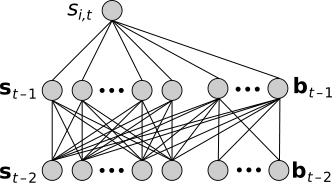
\includegraphics[width=0.45\linewidth]{images/Hidden_Architecture.png}
    \caption{Architecture of the network.}
     \label{fig:net_arch}
\end{figure}

Our aim is to compose a generative model able to reproduce the neural activity of a given dataset. In order to achieve this goal, we will perform a gradient ascent on the likelihood:

\begin{equation}
   \mathcal{L} = \sum_{i t} s_{i}(t) h_{i}(t) - \log{ 2 \, cosh \, h_{i}(t)}
   \label{eq:likelihood}
\end{equation}

In the following section we show the mathematical derivation required for the gradient ascent.


\subsection{Derivatives}

First, we develop the derivative of the likelihood w.r.t. $\*H$ and $\*J$. These derivatives are equal to the ones in the standard Kinetic Ising model:

\begin{align}
    \frac{\partial\mathcal{L}}{\partial H_n} =& \frac{\partial \sum_{it} \left [ s_{i}(t) h_{i}(t) - \log{ 2 \, cosh \, h_{i}(t)} \right ]}{\partial H_n}
    \\ =&  \sum_{t} \left [ s_{n}(t) - tanh \,\left ( h_n(t) \right ) \right ],
\end{align}


\begin{align}
    \frac{\partial\mathcal{L}}{\partial J_{nm}} =& \frac{\partial \sum_{it} \left [ s_{i}(t) h_{i}(t) - \log{ 2 \, cosh \, h_{i}(t)} \right ]}{\partial J_{nm}}
    \\ =& \sum_{t} \left [ s_{n}(t)  s_m(t-1) \right ] - \sum_{it} \left [ \frac{\partial \log{ 2 \, cosh \, h_{i}(t)}}{ \partial J_{nm}} \right ]
    \\ =& \sum_{t} \left [ s_{n}(t) s_m(t-1) \right ] 
    -  \sum_{it} \left [ \frac{\frac{\partial { 2 \, cosh \, h_{i}(t)}}{\partial J_{nm}}}{2 cosh \, h_i(t))} \right ] 
    \\ =& \sum_{t} \left [ s_{n}(t) s_m(t-1) \right ]
    - \sum_{it} \left [  
    \frac{ \frac{ \partial { 2 \, cosh \, h_{i}(t)}}{\partial h_i(t)}\frac{\partial h_i(t)}{\partial J_{nm}}}{
    2 cosh \,h_i(t)}  \right ]
    \\ =& \sum_{t} \left [ s_{n}(t) s_m(t-1)  \right ]
    - \sum_{t} \left [  tanh \,\left ( h_n(t) \right ) s_m(t-1)
    \right ]
    \\ =& \sum_{t} \left [ 
    \left (  s_{n}(t) -  tanh \, h_n(t) \right )
    \left (  s_m(t-1) \right )
    \right ].
\end{align}


Secondly, we derive with respect to $\*M$, resulting in a very similar equation:

\begin{align}
    \frac{\partial\mathcal{L}}{\partial M_{nm}} =& \frac{\partial \sum_{it} \left [ s_{i}(t) h_{i}(t) - \log{ 2 \, cosh \, h_{i}(t)} \right ]}{\partial M_{nm}}
    \\ =& \sum_{t} \left [ s_{n}(t)  b_m(t-1) \right ] - \sum_{it} \left [ \frac{\partial \log{ 2 \, cosh \, h_{i}(t)}}{ \partial M_{nm}} \right ]
    \\ =& \sum_{t} \left [ 
    \left (  s_{n}(t) -  tanh \, h_n(t) \right )\left (  b_m(t-1) \right )
    \right ].
\end{align}

Following we derive w.r.t. $\*K$:

\begin{align}
    \frac{\partial\mathcal{L}}{\partial K_{nm}} =&  \sum_{it} \left [ \frac{ \partial \left ( s_{i}(t) h_{i}(t) - log \, { 2 \, cosh \, h_{i}(t)} \right )}{\partial h_i(t)} \frac{\partial h_i(t)}{\partial K_{nm}} \right ]
    \\ =& \sum_{it} \left [ \left ( s_{i}(t) -  \, tanh \, h_{i}(t) \right ) \frac{\partial h_i(t)}{\partial K_{nm}} \right ]
    \\ =& \sum_{it} \left [ \left ( s_{i}(t) -  \, tanh \, h_{i}(t) \right ) \frac{\partial \left ( \sum_g M_{ig} b_g(t-1) \right ) }{\partial K_{nm}} \right ] 
    \\ =& \sum_{it} \left [ \left ( s_{i}(t) -  \, tanh \, h_{i}(t) \right ) \left ( \sum_g M_{ig} \frac{\partial  b_g(t-1)}{\partial K_{nm}} \right )  \right ],
\end{align}

Having into account that to complete the derivative, we also need to compute the derivative of $b_g(t)$ w.r.t. $\*K$:

\begin{align}
    \frac{\partial b_g(t)}{\partial K_{nm}} 
    =&  \frac{ \partial tanh {\left ( \sum_j K_{gj} s_j(t-1) + \sum_k L_{gk} b_k(t-1) \right )}}{\partial K_{nm}}
    \\ =& \left ( \delta_{gn} \, s_m(t-1) + \sum_k L_{gk} \frac{ \partial b_k(t-1)}{\partial K_{nm}} \right )
    \left ( 1 - b_g^2(t) \right )
\end{align}

Subsequently, we derive the likelihood w.r.t. $\*L$ in a very similar way:

\begin{align}
    \frac{\partial\mathcal{L}}{\partial L_{nm}} =& 
    \sum_{it} \left [ \frac{ \partial \left ( s_{i}(t) h_{i}(t) - \log{ 2 \, cosh \, h_{i}(t)} \right )}{\partial h_i} \frac{\partial h_i}{\partial L_{nm}} \right ]
    \\ =& \sum_{it} \left [ \left ( s_{i}(t) -  \, tanh \, h_{i}(t) \right ) \frac{\partial h_i}{\partial L_{nm}} \right ]
    \\ =& \sum_{it} \left [ \left ( s_{i}(t) -  \, tanh \, h_{i}(t) \right ) \left ( \sum_g M_{ig} \frac{\partial  b_g(t-1)}{\partial L_{nm}} \right )  \right ],
\end{align}

Where the derivative of $b_g(t)$ w.r.t. $\*L$ is:

\begin{align}
    \frac{\partial b_g(t)}{\partial L_{nm}} 
    =&  \frac{ \partial tanh {\left ( \sum_j K_{gj} s_j(t-1) + \sum_k L_{gk} b_k(t-1) \right )}}{\partial L_{nm}}
    \\ =& \left ( \delta_{gn} \, b_m(t-1) + \sum_k  L_{gk} \frac{ \partial b_k(t-1)}{\partial L_{nm}}\right ) \left ( 1 - b_g^2(t) \right )
\end{align}

Finally, to avoid a cold start setting $b(t=0)$ to 0, we define the derivative of the likelihood w.r.t. $\*b(t=0)$
\begin{align}
    \frac{\partial\mathcal{L}}{\partial b_{z}(0)} =& \frac{\partial \sum_{it} \left [ s_{i}(t) h_{i}(t) - \log{ 2 \, cosh \, h_{i}(t)} \right ]}{\partial b_{z}(0)}
    \\ = & \frac{\partial \sum_{i} \left [ s_{i}(1) h_{i}(t) - \log{ 2 \, cosh \, h_{i}(1)} \right ]}{\partial b_{z}(0)}
    + \frac{\partial \sum_{i} \left [ s_{i}(2) h_{i}(2) - \log{ 2 \, cosh \, h_{i}(2)} \right ]}{\partial b_{z}(0)}
     \\ =& \sum_{i}  \left ( s_{i}(1) - tanh \, h_{i}(1) \right )  M_{iz}
     + \sum_{i}  \left ( s_{i}(2) - tanh \, h_{i}(2) \right )  
     \left ( \sum_g M_{ig} (1 - b_g^2(1)) L_{gz
     } \right )
\end{align}

\section{Results}

To test our method, we compare the performance of our method in contrast to the standard Kinetic Ising model. We are interested in a scenario in which there is a model generating data but only a portion of these data is visible to the models. To reproduce this, we first simulate a model with N=10 total neurons for 5000 steps where we only collect the data from V=6 visible neurons. Subsequently, we try to infer the parameters that maximize the likelihood both with a standard Kinetic Ising model and with a Kinetic Ising model with a unique hidden unit. We asses the inference process doing a simulation of the network every 250 iterations for 6500 time-steps. With the data generated in the simulations, we compute the mean ($\*m$), same time correlations ($\*C$) and delayed correlations ($\*D$).\\

In order to make sure that the results were not biased by the initialization of each of the algorithms, we have repeated the experiments several times randomly modifying several aspects driven with a seed. These aspects include: the parameters $\*H$ and $\*J$ of the original model, the random selection of the neurons out of the original set and the initialization of the parameters of the new models.\\

In all the figures displayed in the appendix~\ref{sec:figures} we can observe the same behavior. If we look at the bottom part of the figures we will see that the Mean Squared Error (MSE) of the all the statistical moments $\*m$,  $\*C$ and  $\*D$ computed after the simulations is always lower or equal in the models with a hidden unit. This is more remarkable in most of the cases if we observe the MSE of the mean and the delayed correlations. The results can be reproduced using the script sim\_fit\_HI2.py and modifying the seed. 


\bibliographystyle{unsrt}
\bibliography{references}

\newpage
\appendix
\section{Figures}
\label{sec:figures}

\subsection{Seed 722}

\begin{figure}[!htb]
    \centering
    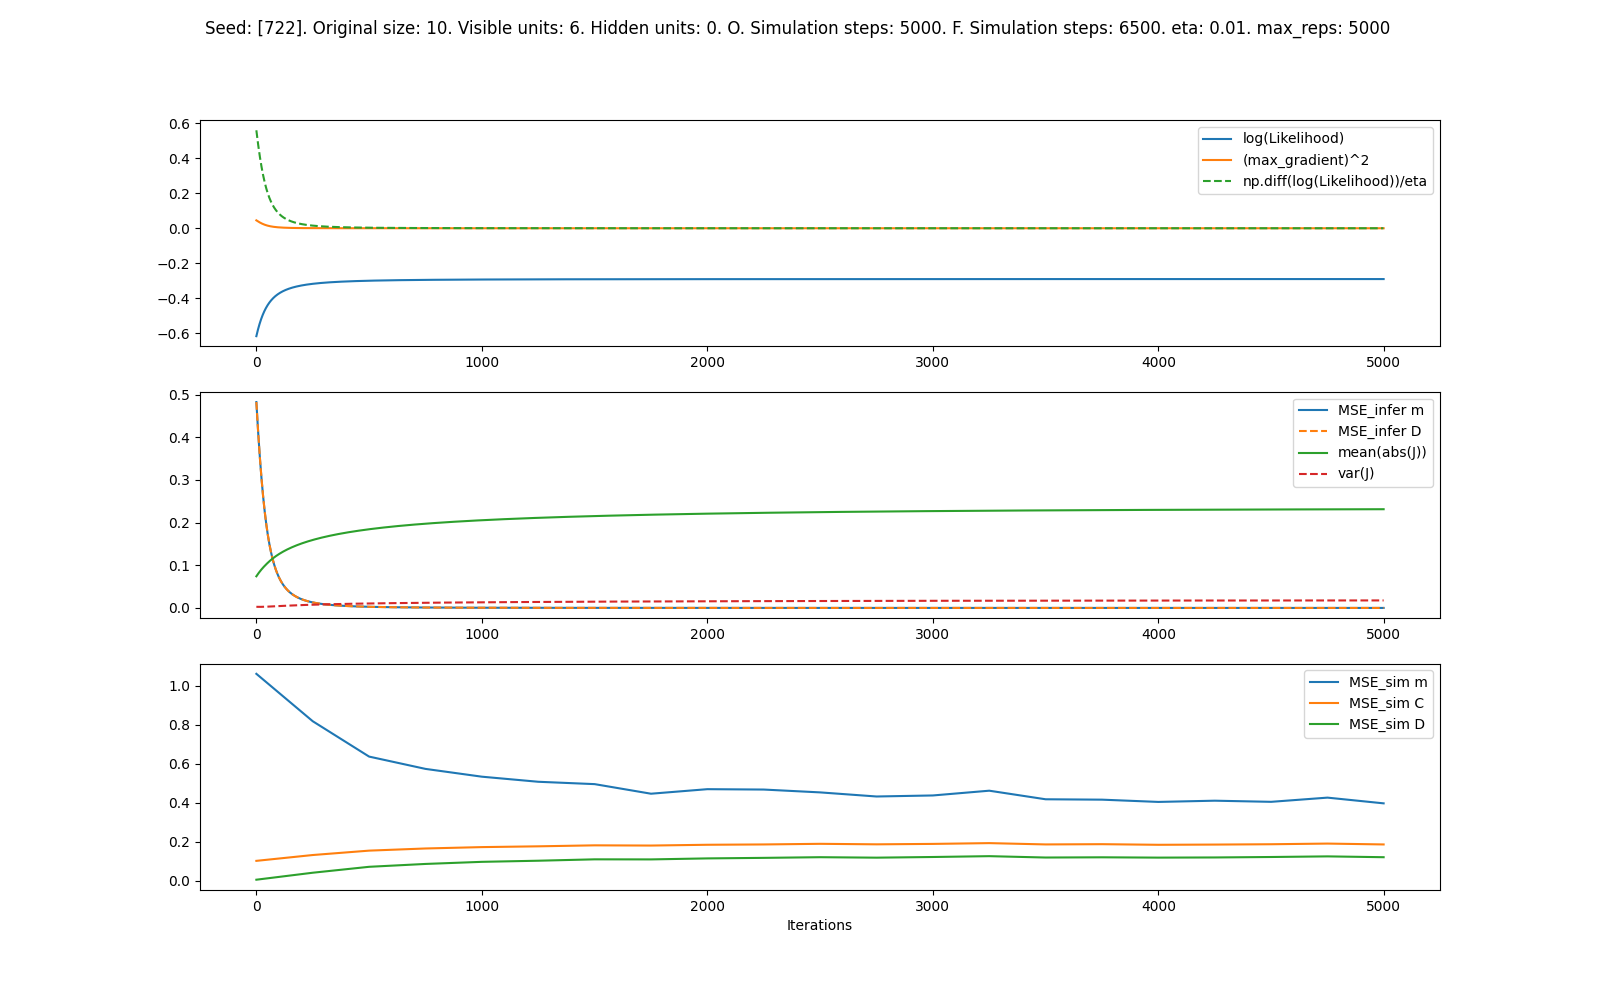
\includegraphics[width=0.7\linewidth]{images/sqrt_size/[722]_10_6_0_5000_6500_eta001_5000_100.png}
\caption{Seed: 722. Standard Ising model. Top: logarithm of the likelihood, square of the maximum gradient and difference of the likelihood between consecutive time-steps. Middle: MSE of m and D during inference and evolution of the behavior of $\*J$. Bottom: MSE of m, D and D after the simulations.}
\end{figure}


\begin{figure}[!htb]
    \centering
    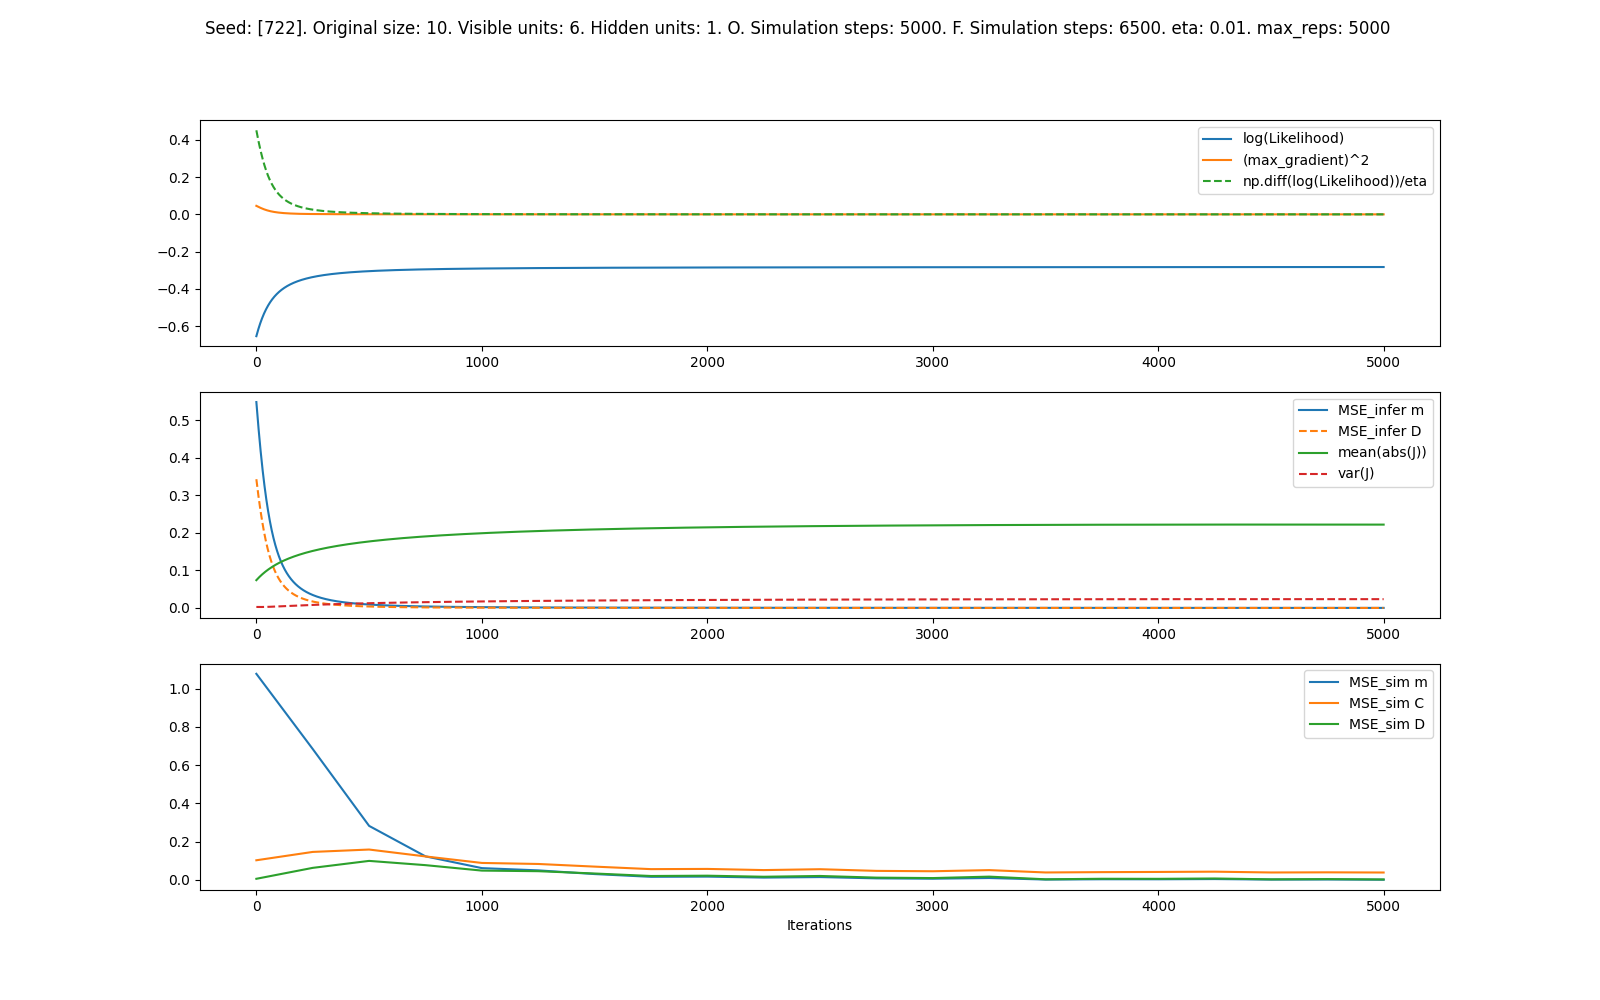
\includegraphics[width=0.7\linewidth]{images/sqrt_size/[722]_10_6_1_5000_6500_eta001_5000_100.png}
\caption{Seed: 722. Kinetic Ising model with 1 hidden unit. Top: logarithm of the likelihood, square of the maximum gradient and difference of the likelihood between consecutive time-steps. Middle: MSE of m and D during inference and evolution of the behavior of $\*J$. Bottom: MSE of m, D and D after the simulations.}
\end{figure}


\newpage
\subsection{Seed 1185}

\begin{figure}[!htb]
    \centering
    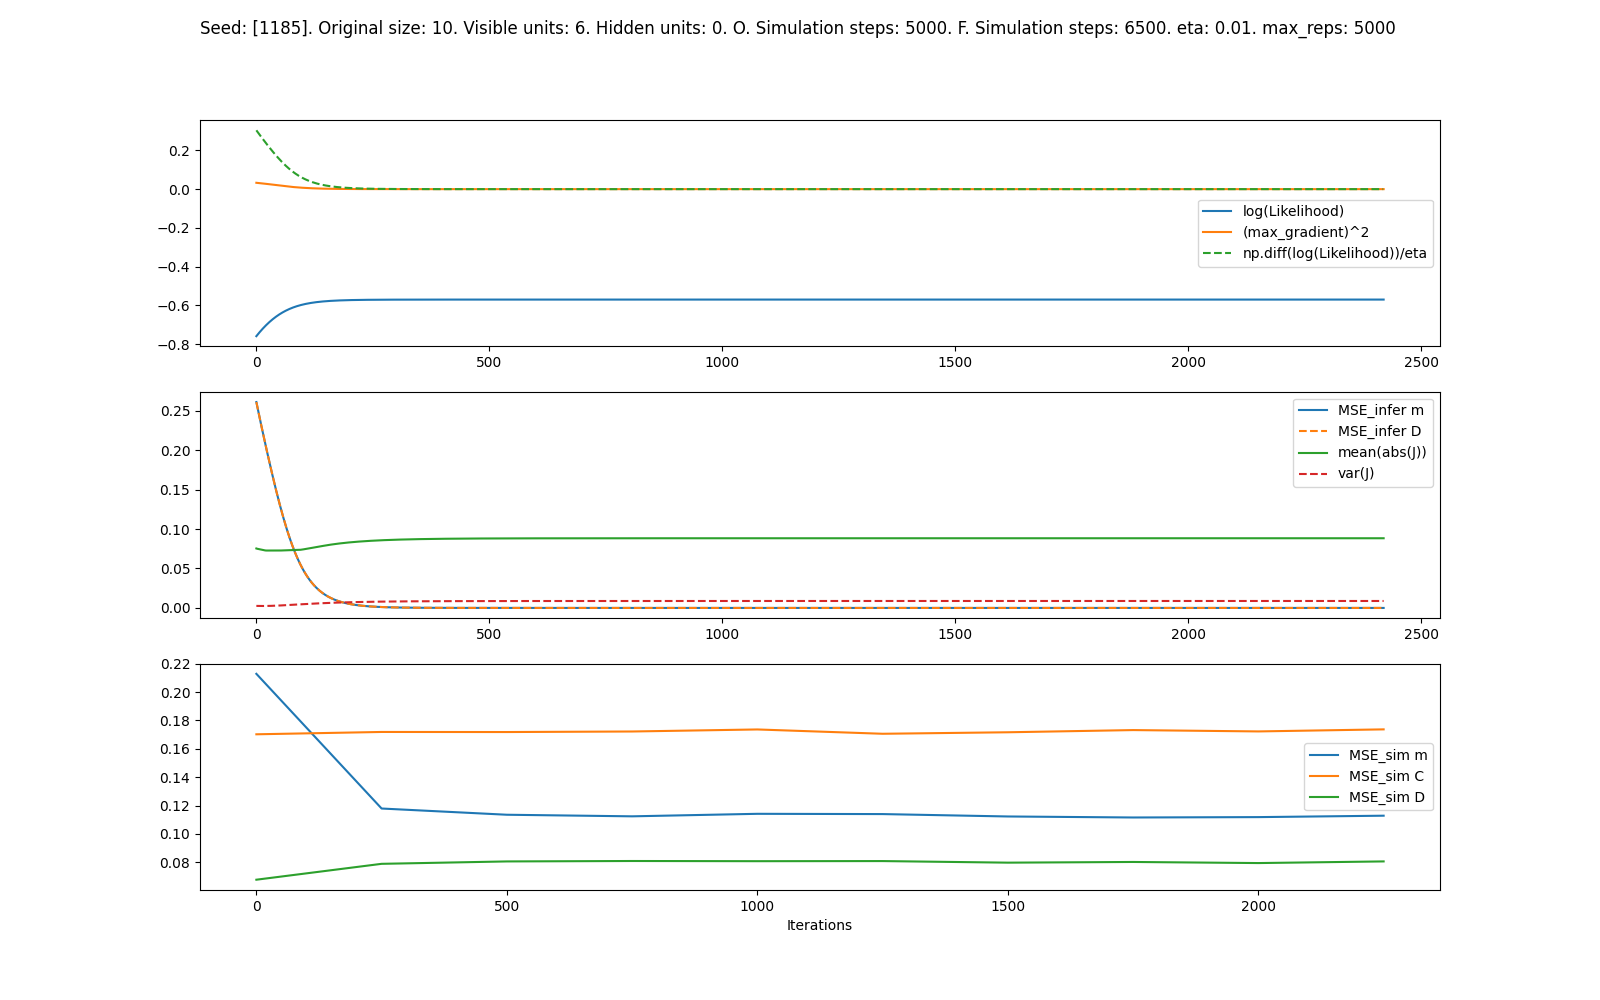
\includegraphics[width=0.7\linewidth]{images/sqrt_size/[1185]_10_6_0_5000_6500_eta001_5000_100.png}
\caption{Seed: 1185. Standard Ising model. Top: logarithm of the likelihood, square of the maximum gradient and difference of the likelihood between consecutive time-steps. Middle: MSE of m and D during inference and evolution of the behavior of $\*J$. Bottom: MSE of m, D and D after the simulations.}
\end{figure}


\begin{figure}[!htb]
    \centering
    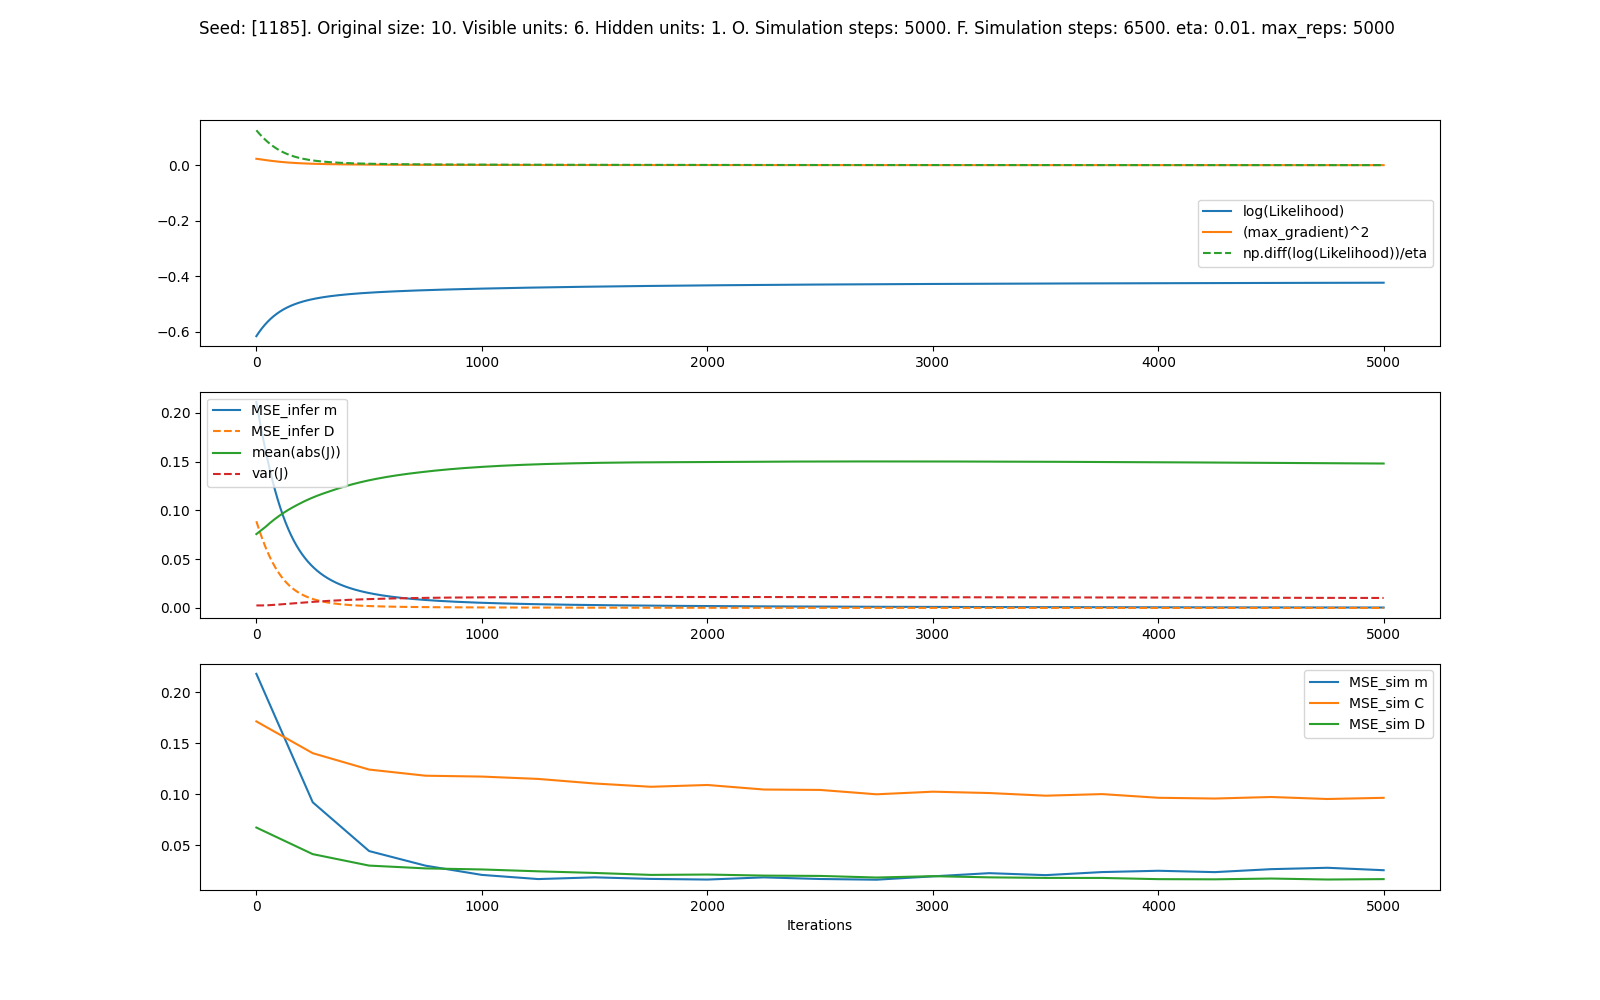
\includegraphics[width=0.7\linewidth]{images/sqrt_size/[1185]_10_6_1_5000_6500_eta001_5000_100.png}
\caption{Seed: 1185. Kinetic Ising model with 1 hidden unit. Top: logarithm of the likelihood, square of the maximum gradient and difference of the likelihood between consecutive time-steps. Middle: MSE of m and D during inference and evolution of the behavior of $\*J$. Bottom: MSE of m, D and D after the simulations.}
\end{figure}


\newpage
\subsection{Seed 2178}

\begin{figure}[!htb]
    \centering
    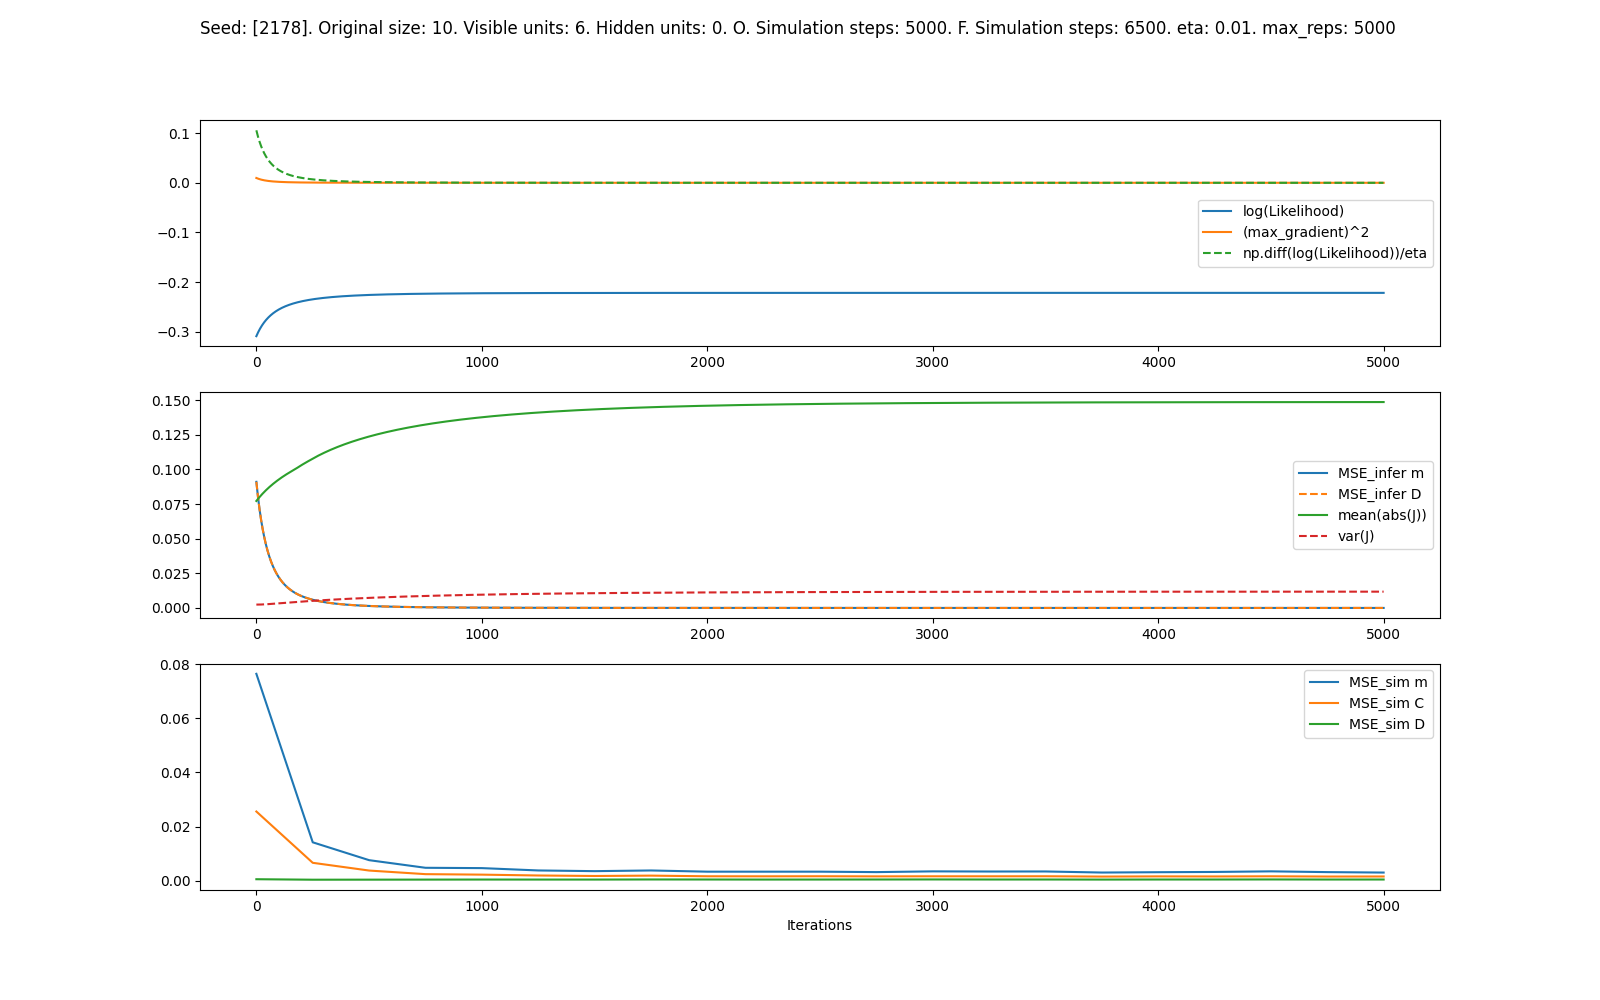
\includegraphics[width=0.7\linewidth]{images/sqrt_size/[2178]_10_6_0_5000_6500_eta001_5000_100.png}
\caption{Seed: 2178. Standard Ising model. Top: logarithm of the likelihood, square of the maximum gradient and difference of the likelihood between consecutive time-steps. Middle: MSE of m and D during inference and evolution of the behavior of $\*J$. Bottom: MSE of m, D and D after the simulations.}
\end{figure}


\begin{figure}[!htb]
    \centering
    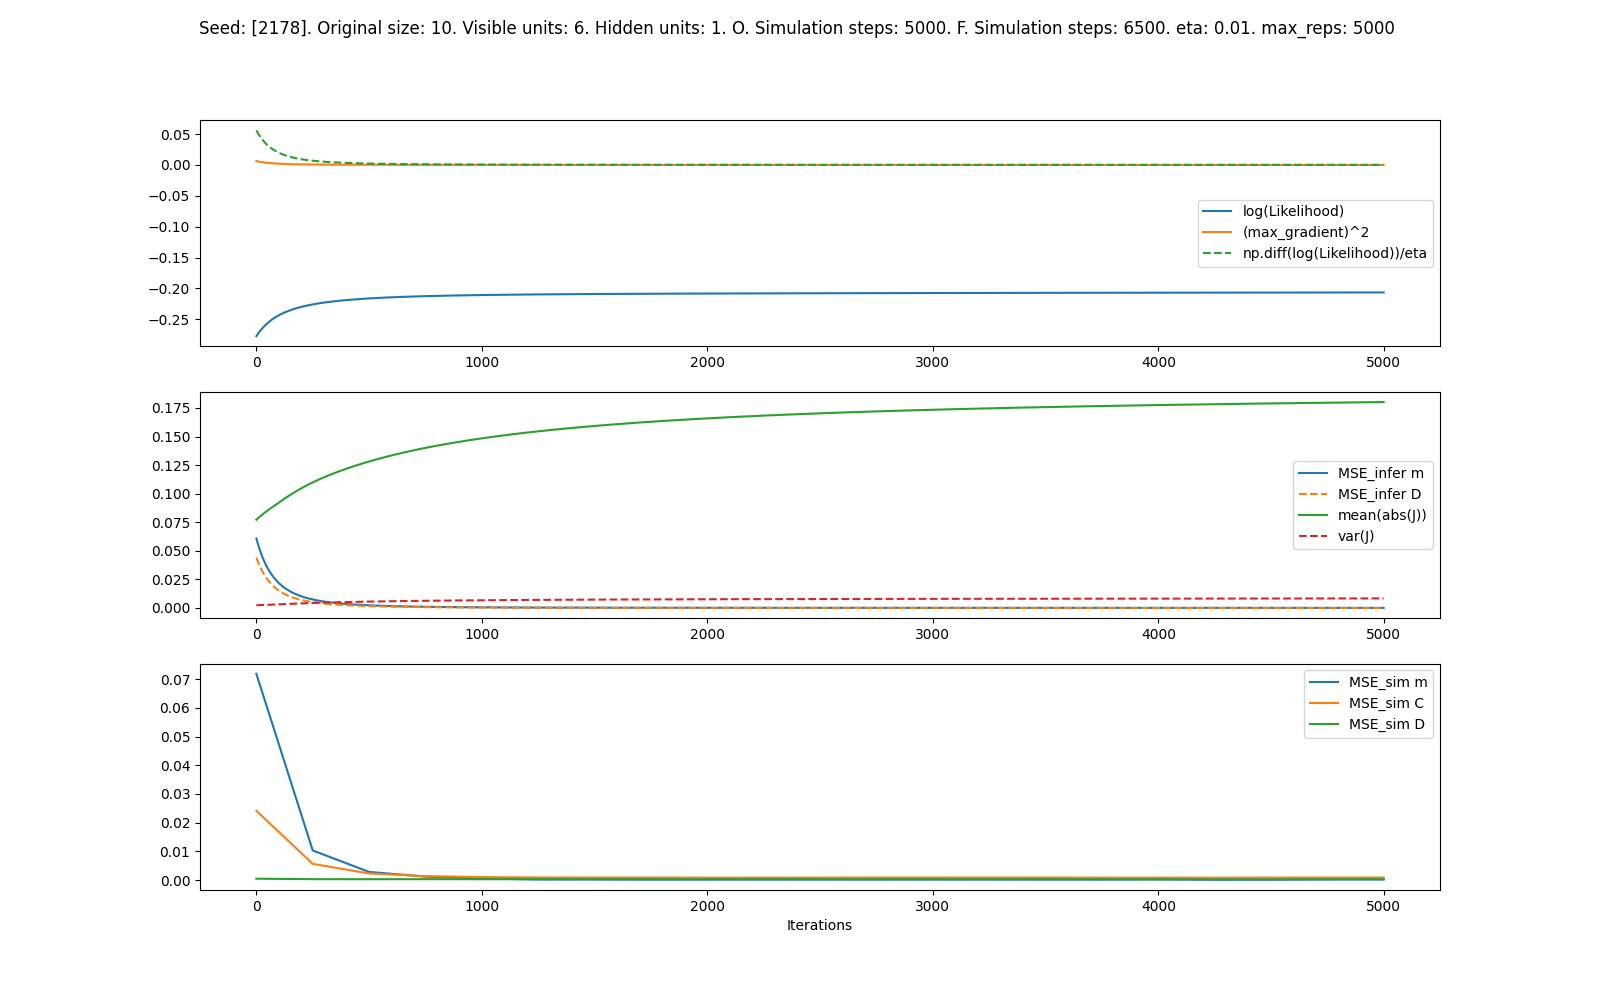
\includegraphics[width=0.7\linewidth]{images/sqrt_size/[2178]_10_6_1_5000_6500_eta001_5000_100.png}
\caption{Seed: 2178. Kinetic Ising model with 1 hidden unit. Top: logarithm of the likelihood, square of the maximum gradient and difference of the likelihood between consecutive time-steps. Middle: MSE of m and D during inference and evolution of the behavior of $\*J$. Bottom: MSE of m, D and D after the simulations.}
\end{figure}



\newpage
\subsection{Seed 2692}

\begin{figure}[!htb]
    \centering
    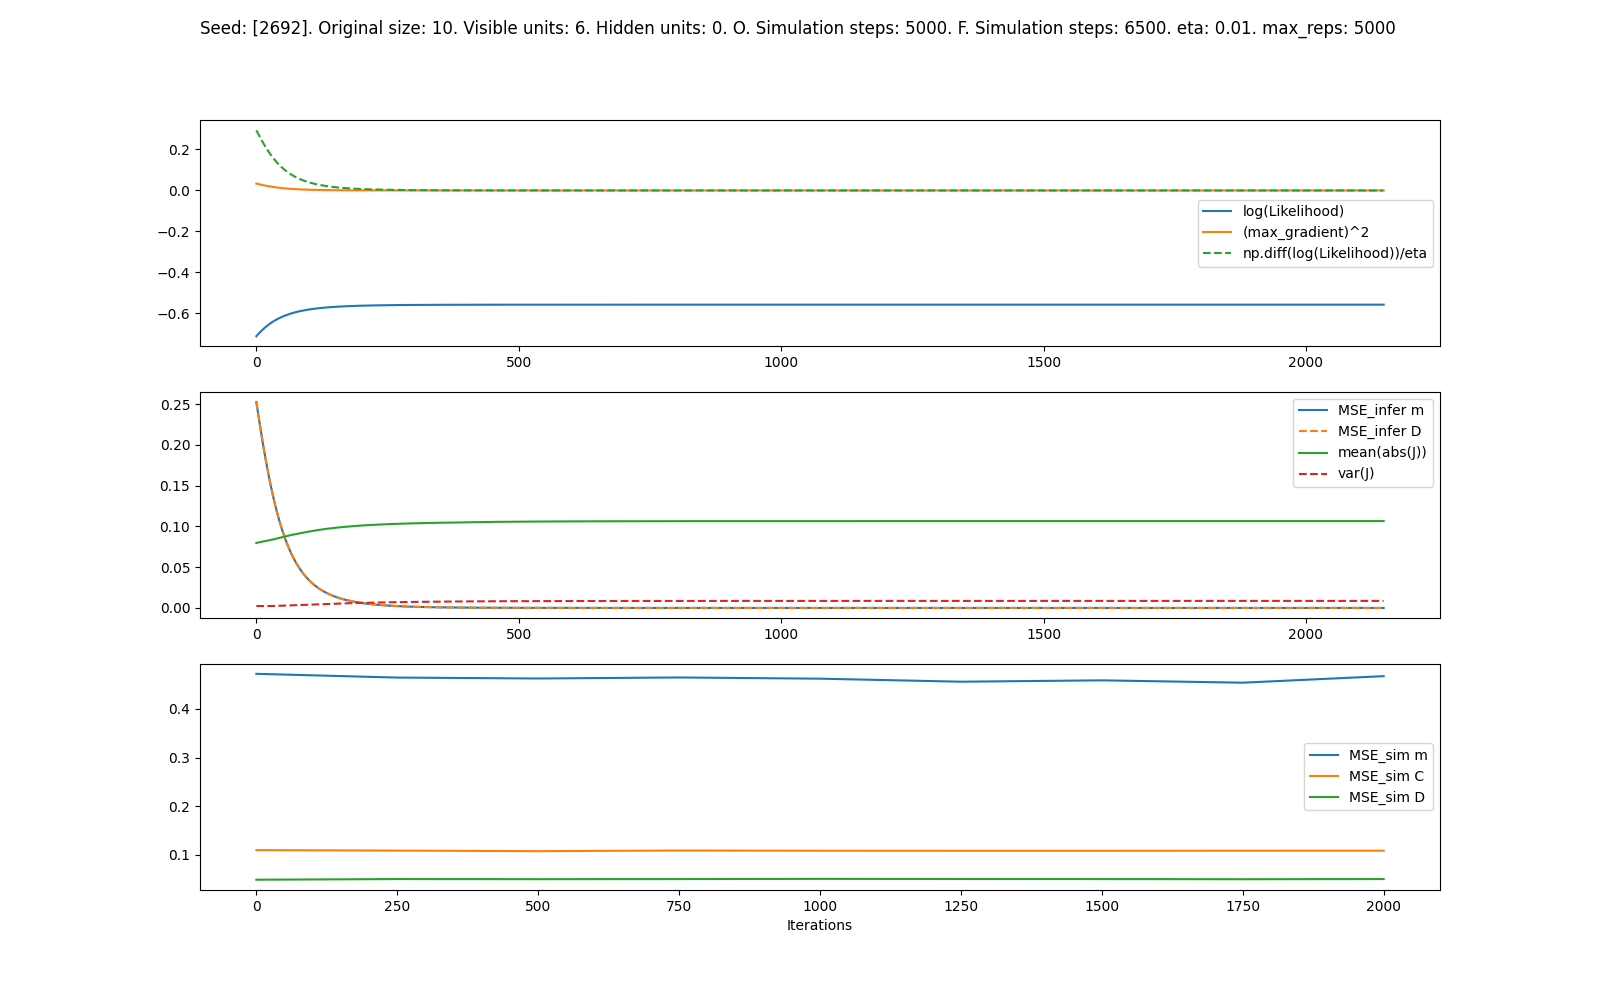
\includegraphics[width=0.7\linewidth]{images/sqrt_size/[2692]_10_6_0_5000_6500_eta001_5000_100.png}
\caption{Seed: 2692. Standard Ising model. Top: logarithm of the likelihood, square of the maximum gradient and difference of the likelihood between consecutive time-steps. Middle: MSE of m and D during inference and evolution of the behavior of $\*J$. Bottom: MSE of m, D and D after the simulations.}
\end{figure}


\begin{figure}[!htb]
    \centering
    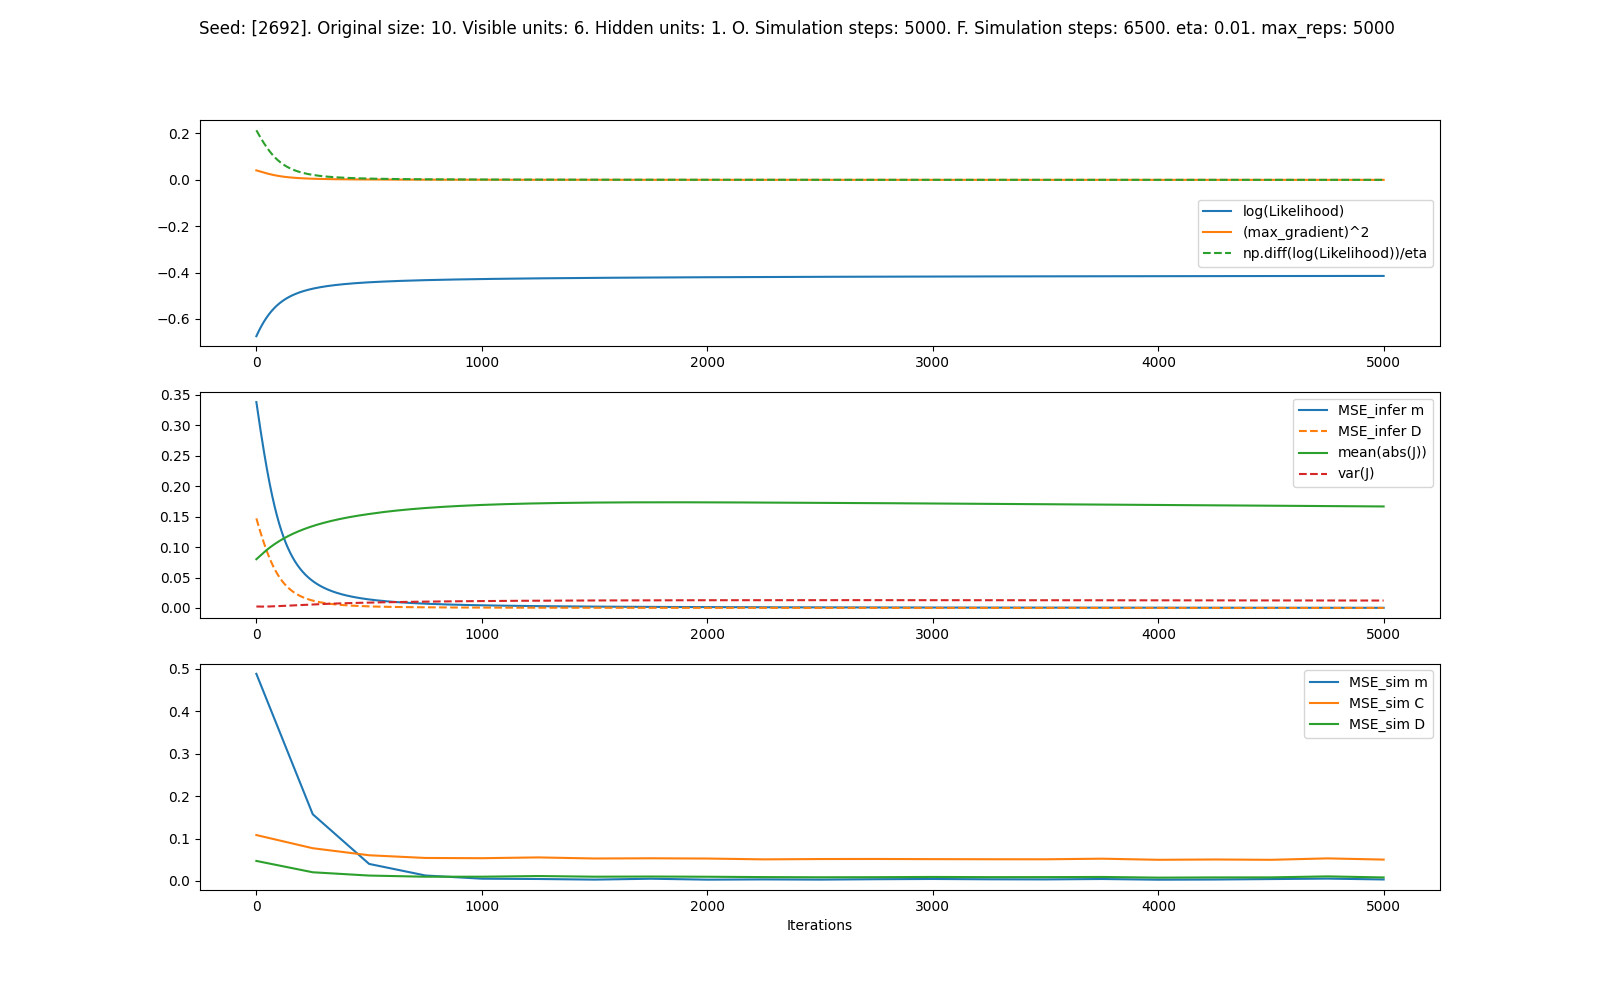
\includegraphics[width=0.7\linewidth]{images/sqrt_size/[2692]_10_6_1_5000_6500_eta001_5000_100.png}
\caption{Seed: 2692. Kinetic Ising model with 1 hidden unit. Top: logarithm of the likelihood, square of the maximum gradient and difference of the likelihood between consecutive time-steps. Middle: MSE of m and D during inference and evolution of the behavior of $\*J$. Bottom: MSE of m, D and D after the simulations.}
\end{figure}



\newpage
\subsection{Seed 3262}

\begin{figure}[!htb]
    \centering
    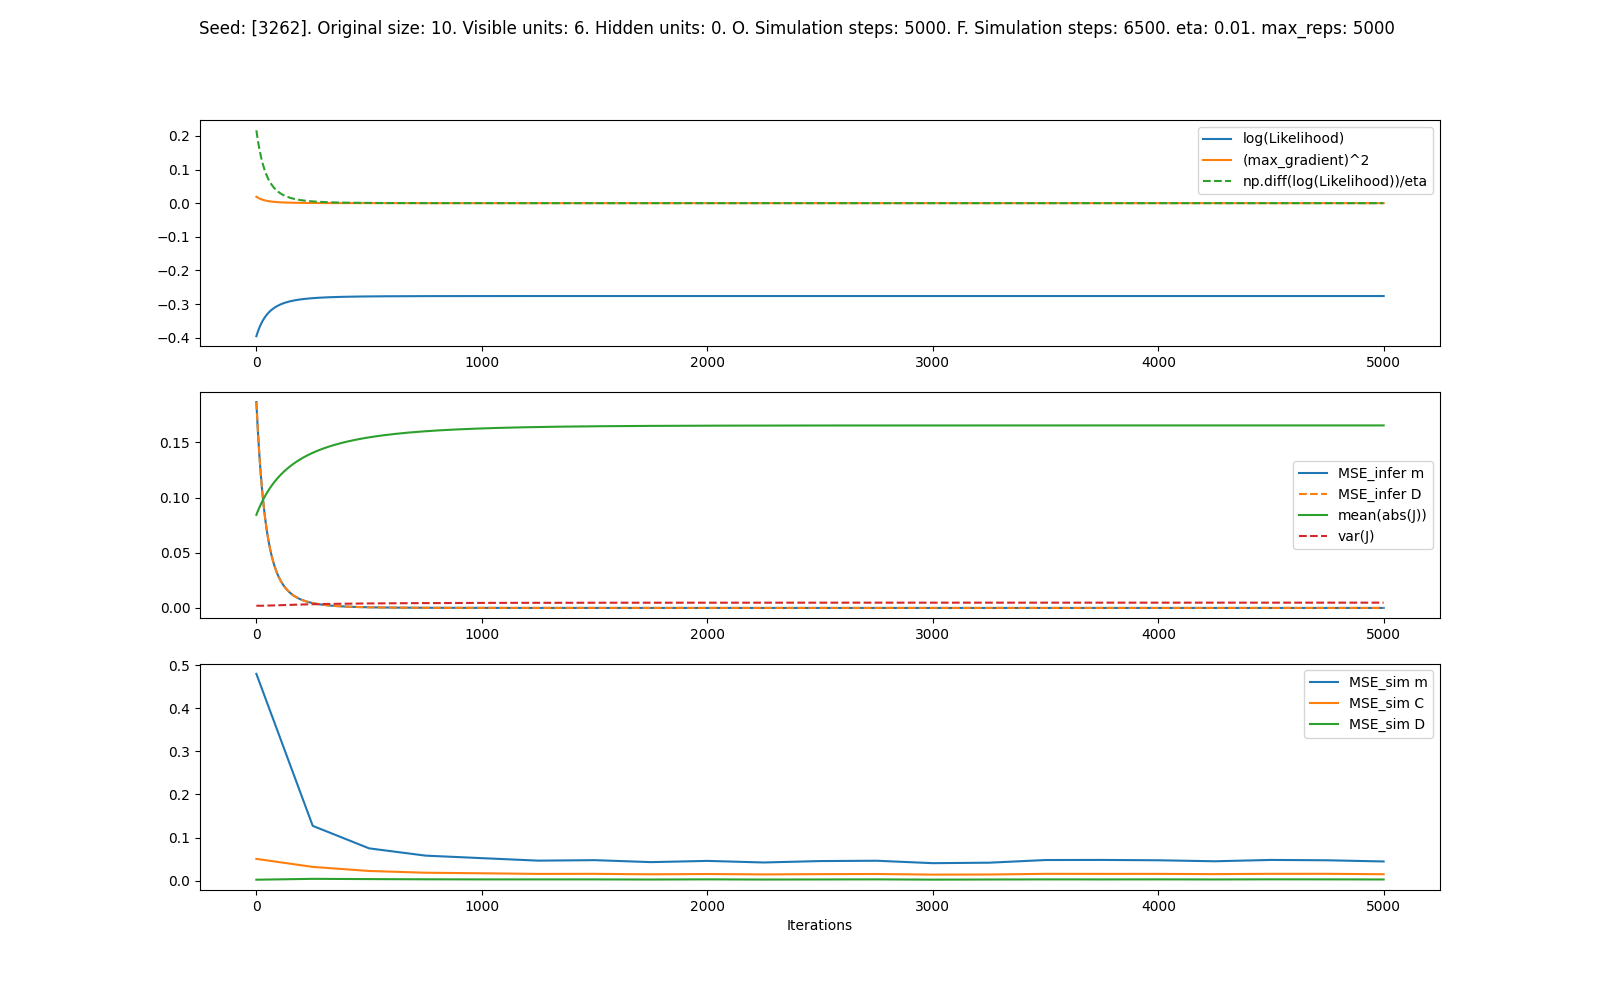
\includegraphics[width=0.7\linewidth]{images/sqrt_size/[3262]_10_6_0_5000_6500_eta001_5000_100.png}
\caption{Seed: 3262. Standard Ising model. Top: logarithm of the likelihood, square of the maximum gradient and difference of the likelihood between consecutive time-steps. Middle: MSE of m and D during inference and evolution of the behavior of $\*J$. Bottom: MSE of m, D and D after the simulations.}
\end{figure}


\begin{figure}[!htb]
    \centering
    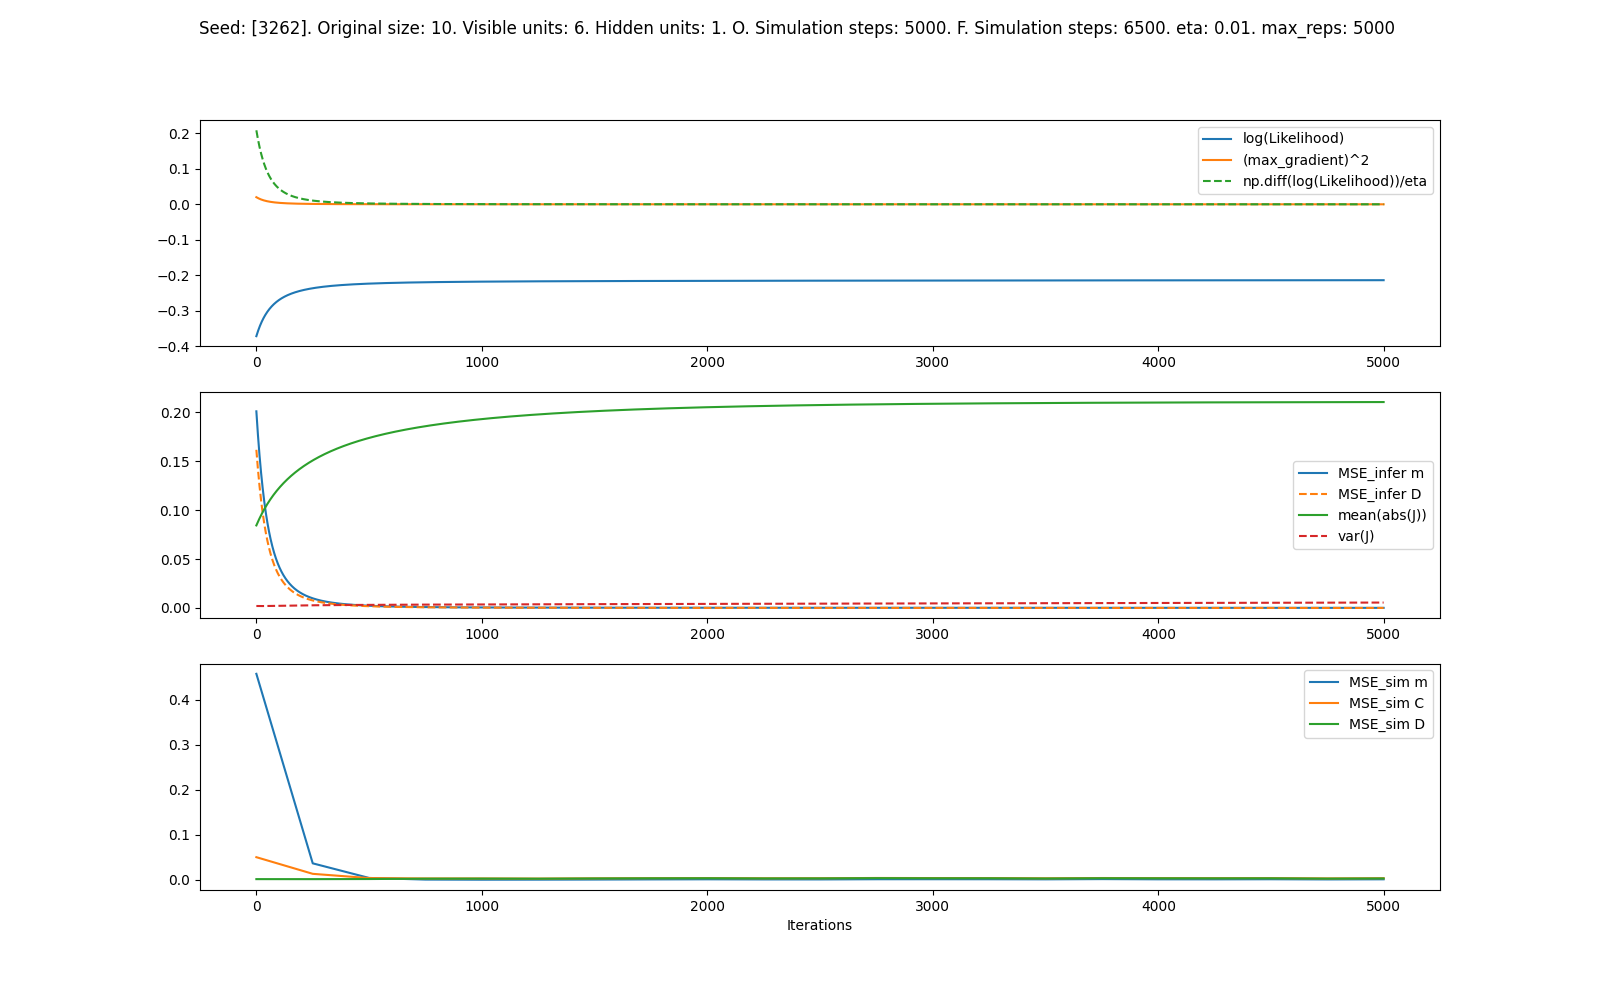
\includegraphics[width=0.7\linewidth]{images/sqrt_size/[3262]_10_6_1_5000_6500_eta001_5000_100.png}
\caption{Seed: 3262. Kinetic Ising model with 1 hidden unit. Top: logarithm of the likelihood, square of the maximum gradient and difference of the likelihood between consecutive time-steps. Middle: MSE of m and D during inference and evolution of the behavior of $\*J$. Bottom: MSE of m, D and D after the simulations.}
\end{figure}



\newpage
\subsection{Seed 3813}

\begin{figure}[!htb]
    \centering
    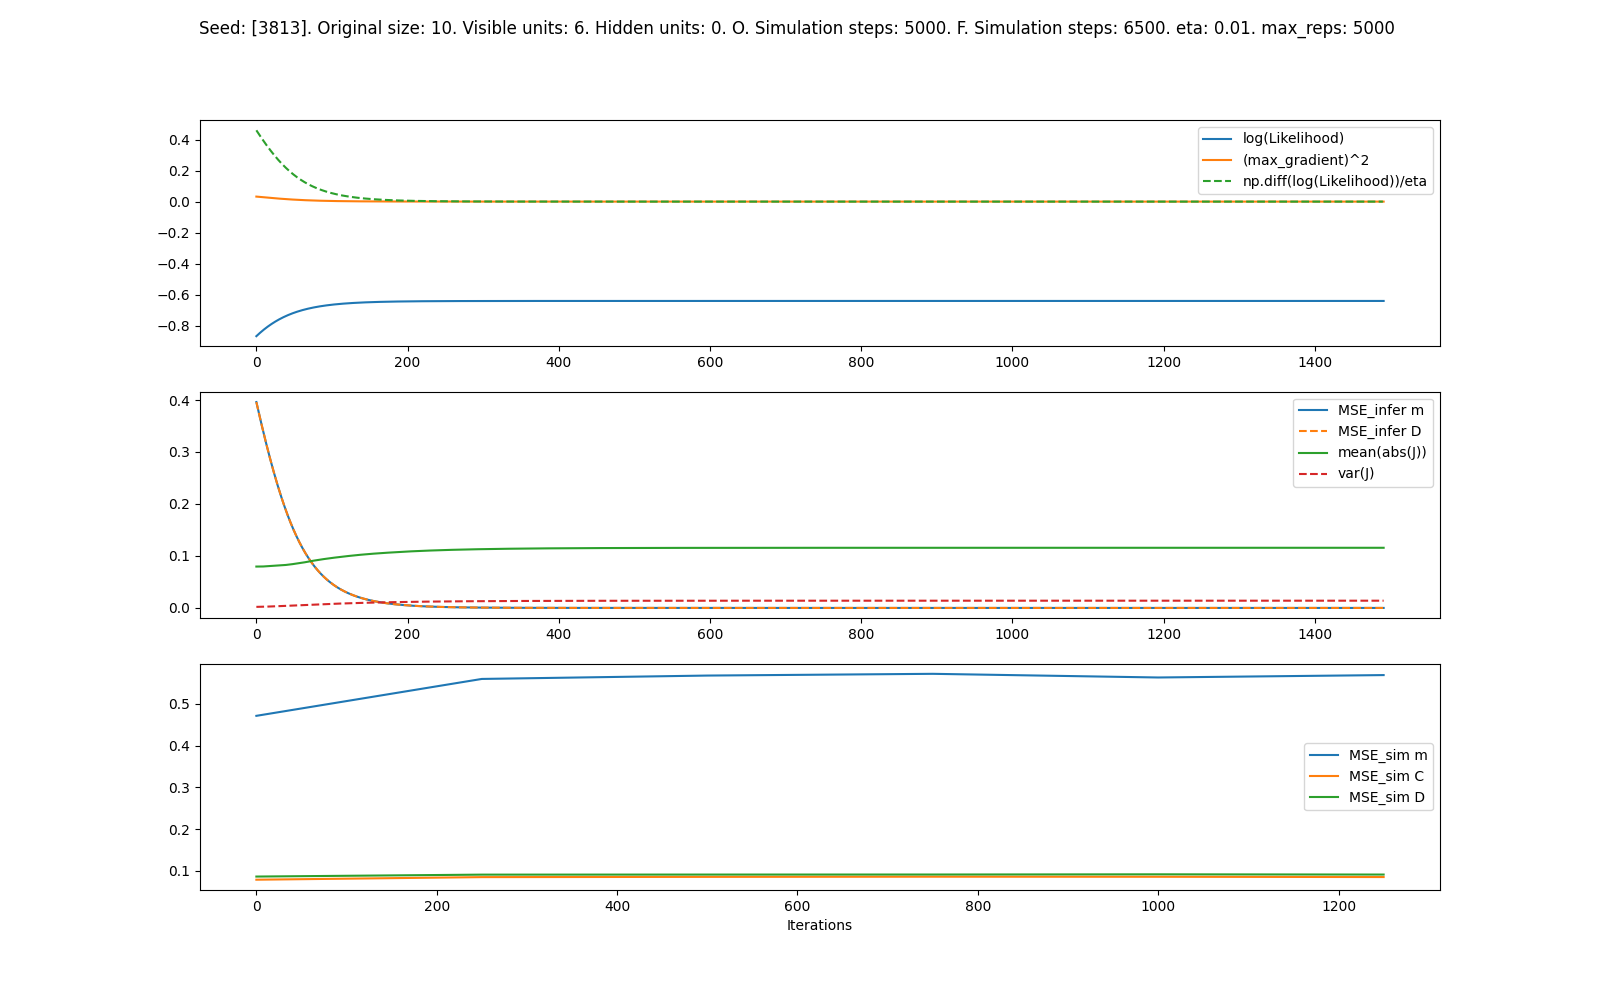
\includegraphics[width=0.7\linewidth]{images/sqrt_size/[3813]_10_6_0_5000_6500_eta001_5000_100.png}
\caption{Seed: 3813. Standard Ising model. Top: logarithm of the likelihood, square of the maximum gradient and difference of the likelihood between consecutive time-steps. Middle: MSE of m and D during inference and evolution of the behavior of $\*J$. Bottom: MSE of m, D and D after the simulations.}
\end{figure}


\begin{figure}[!htb]
    \centering
    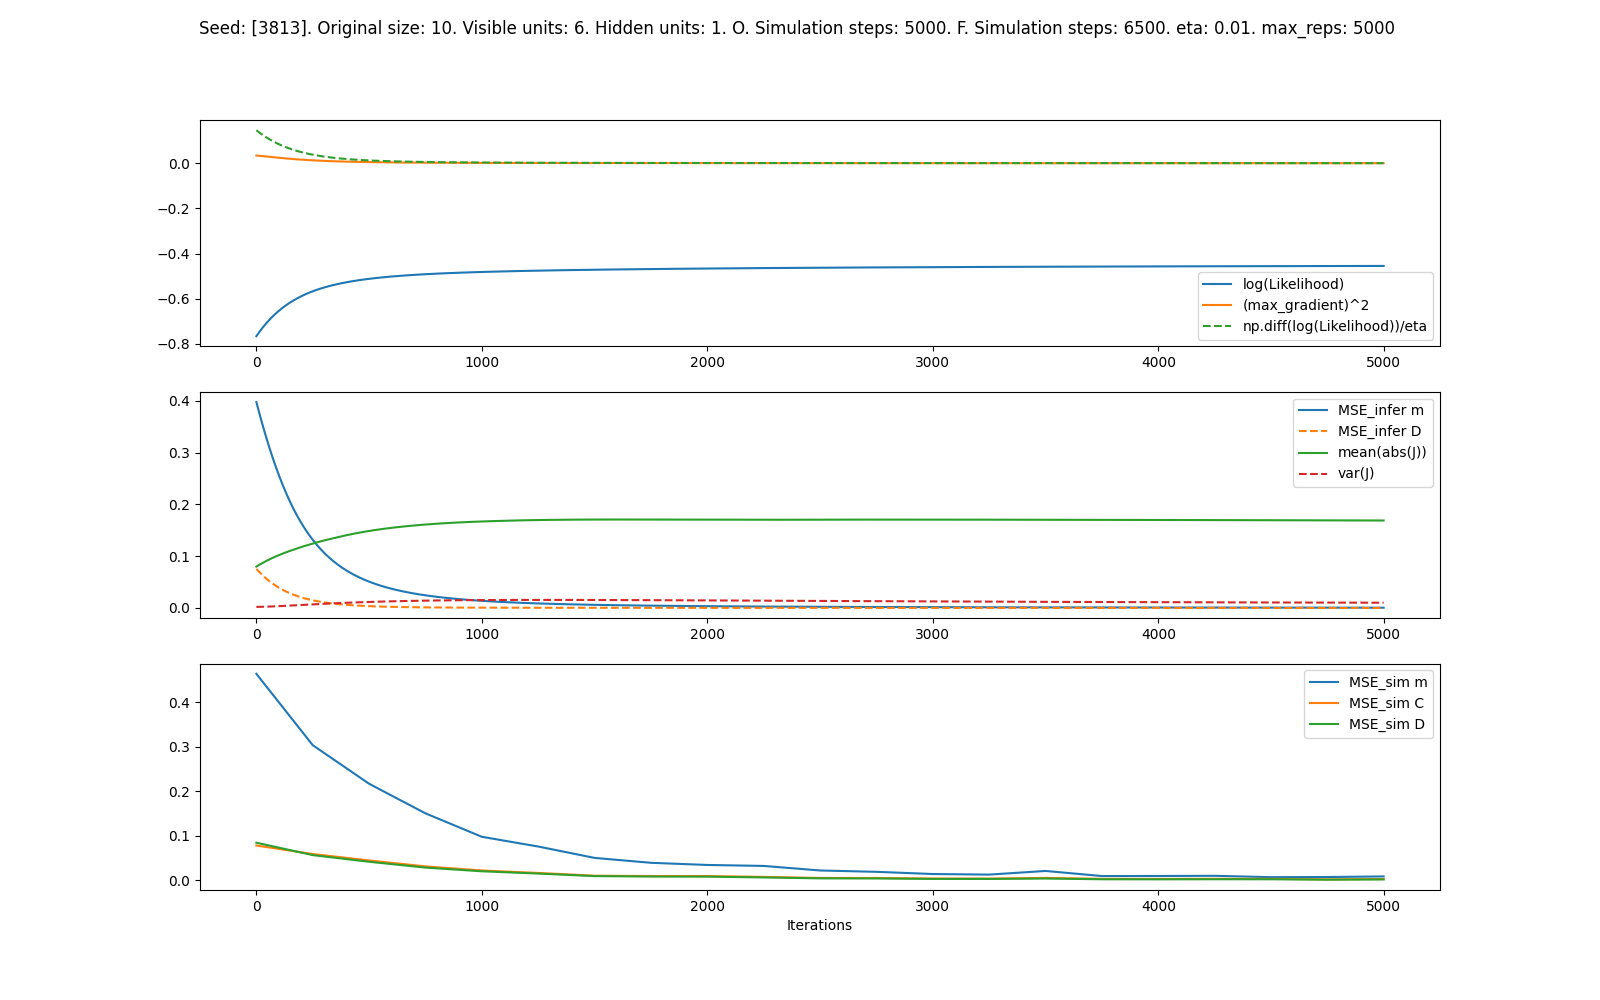
\includegraphics[width=0.7\linewidth]{images/sqrt_size/[3813]_10_6_1_5000_6500_eta001_5000_100.png}
\caption{Seed: 3813. Kinetic Ising model with 1 hidden unit. Top: logarithm of the likelihood, square of the maximum gradient and difference of the likelihood between consecutive time-steps. Middle: MSE of m and D during inference and evolution of the behavior of $\*J$. Bottom: MSE of m, D and D after the simulations.}
\end{figure}



\newpage
\subsection{Seed 3988}

\begin{figure}[!htb]
    \centering
    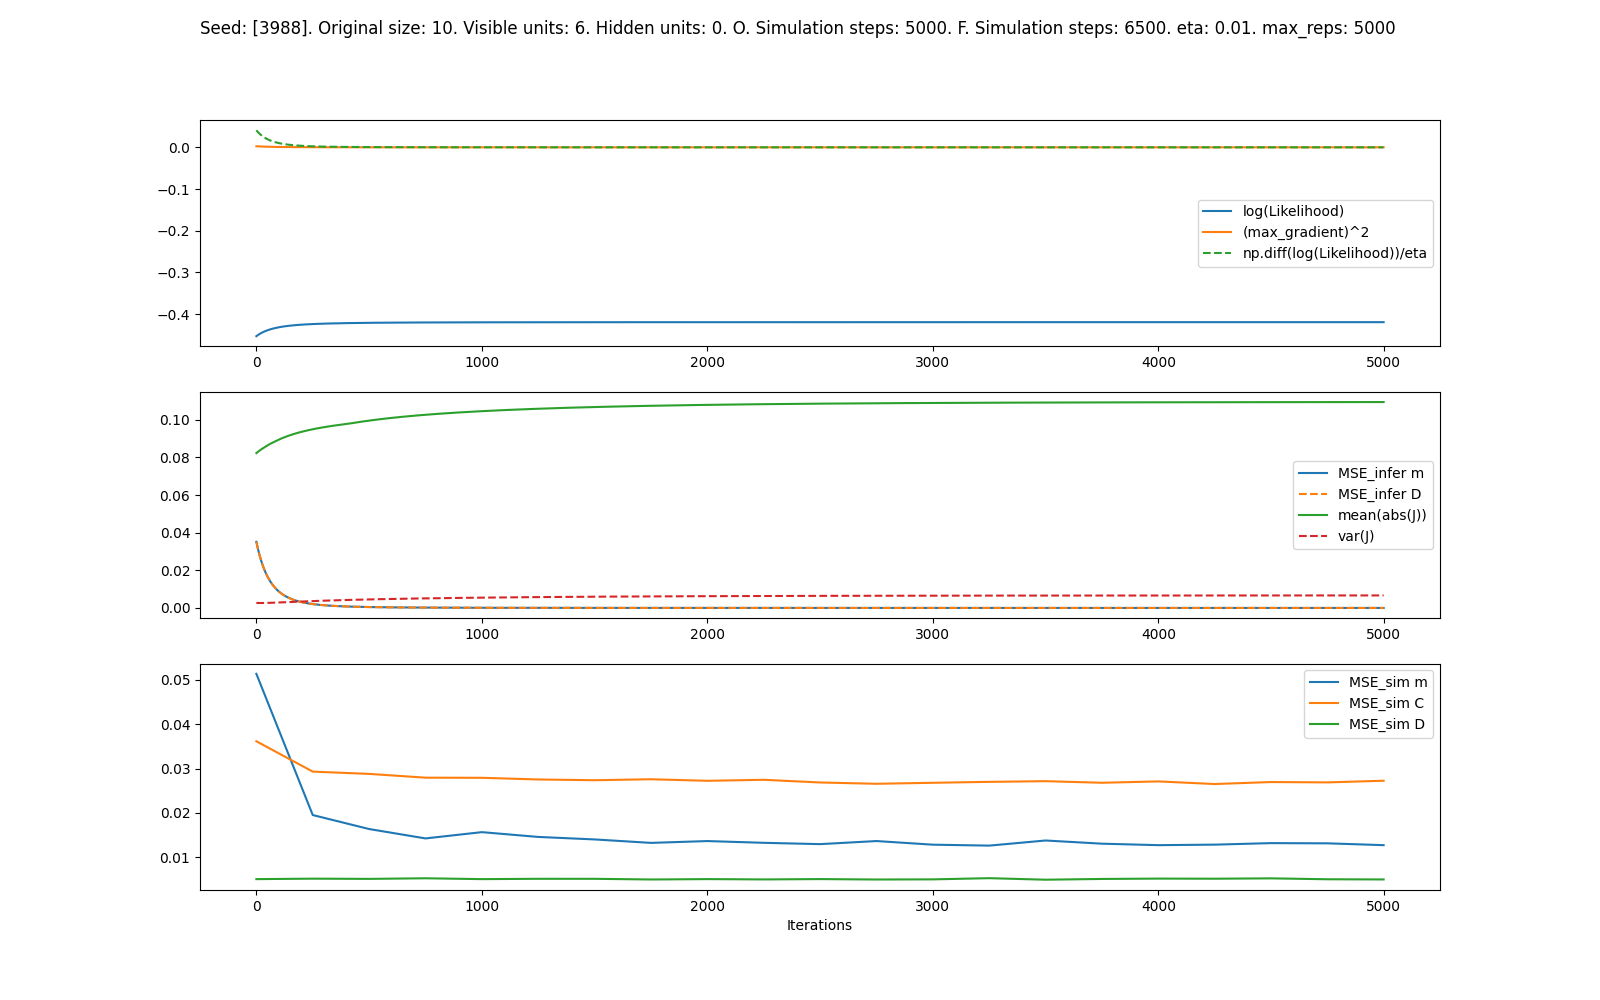
\includegraphics[width=0.7\linewidth]{images/sqrt_size/[3988]_10_6_0_5000_6500_eta001_5000_100.png}
\caption{Seed: 3988. Standard Ising model. Top: logarithm of the likelihood, square of the maximum gradient and difference of the likelihood between consecutive time-steps. Middle: MSE of m and D during inference and evolution of the behavior of $\*J$. Bottom: MSE of m, D and D after the simulations.}
\end{figure}


\begin{figure}[!htb]
    \centering
    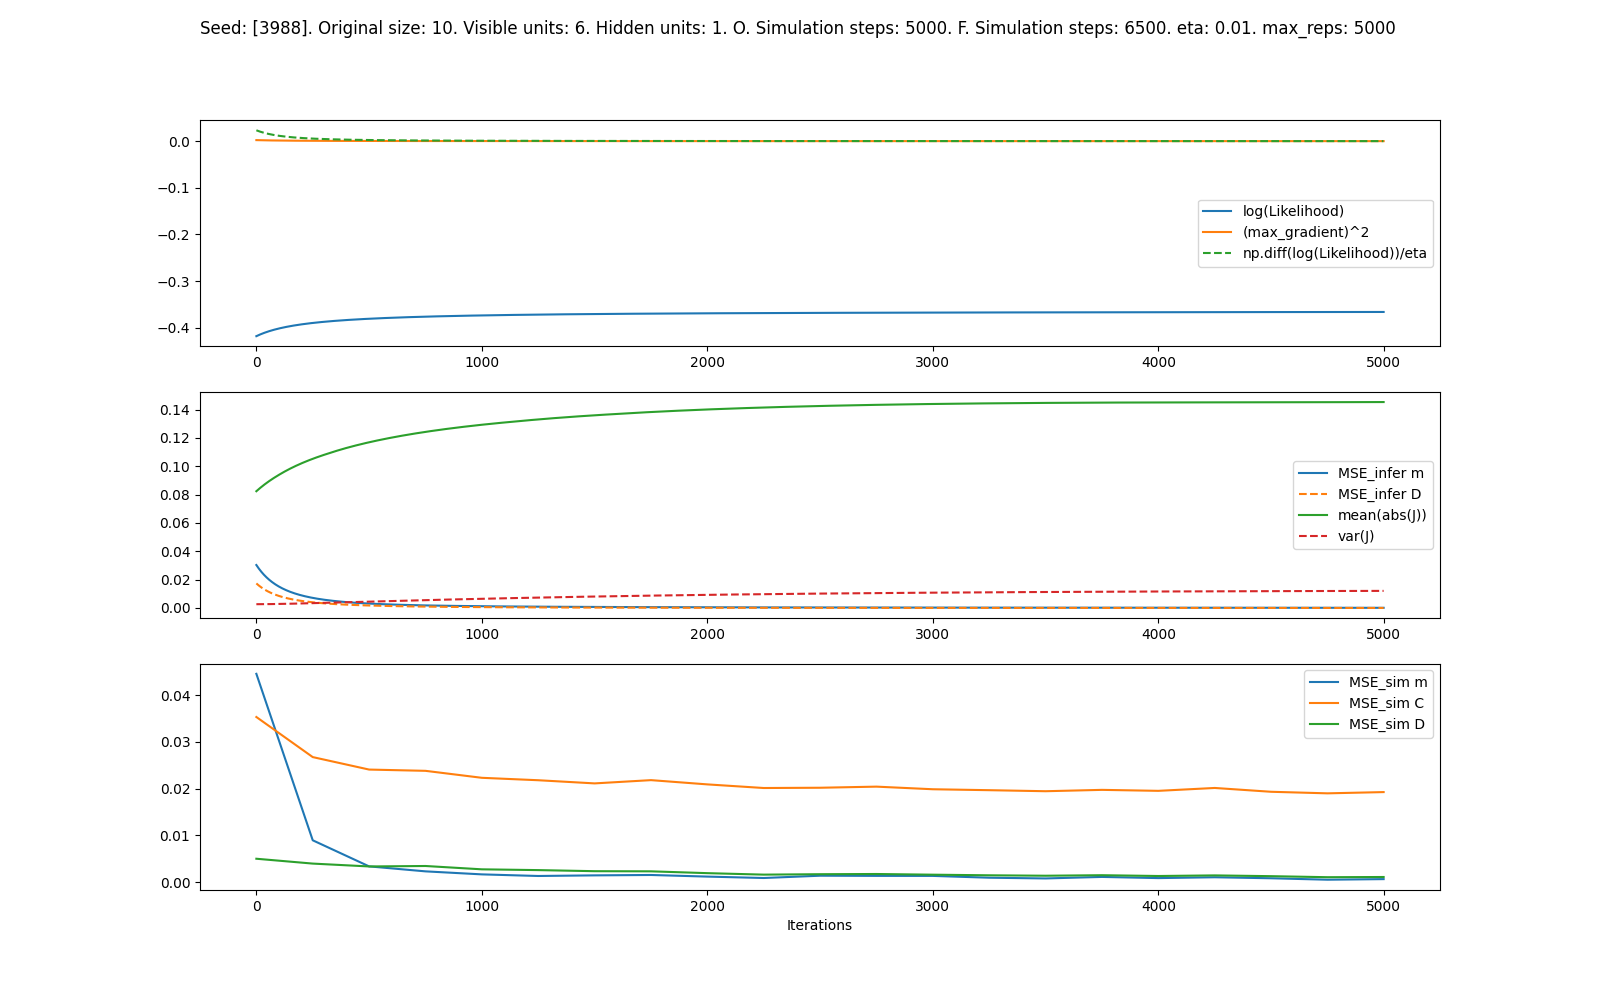
\includegraphics[width=0.7\linewidth]{images/sqrt_size/[3988]_10_6_1_5000_6500_eta001_5000_100.png}
\caption{Seed: 3988. Kinetic Ising model with 1 hidden unit. Top: logarithm of the likelihood, square of the maximum gradient and difference of the likelihood between consecutive time-steps. Middle: MSE of m and D during inference and evolution of the behavior of $\*J$. Bottom: MSE of m, D and D after the simulations.}
\end{figure}





\newpage
\subsection{Seed 4075}

\begin{figure}[!htb]
    \centering
    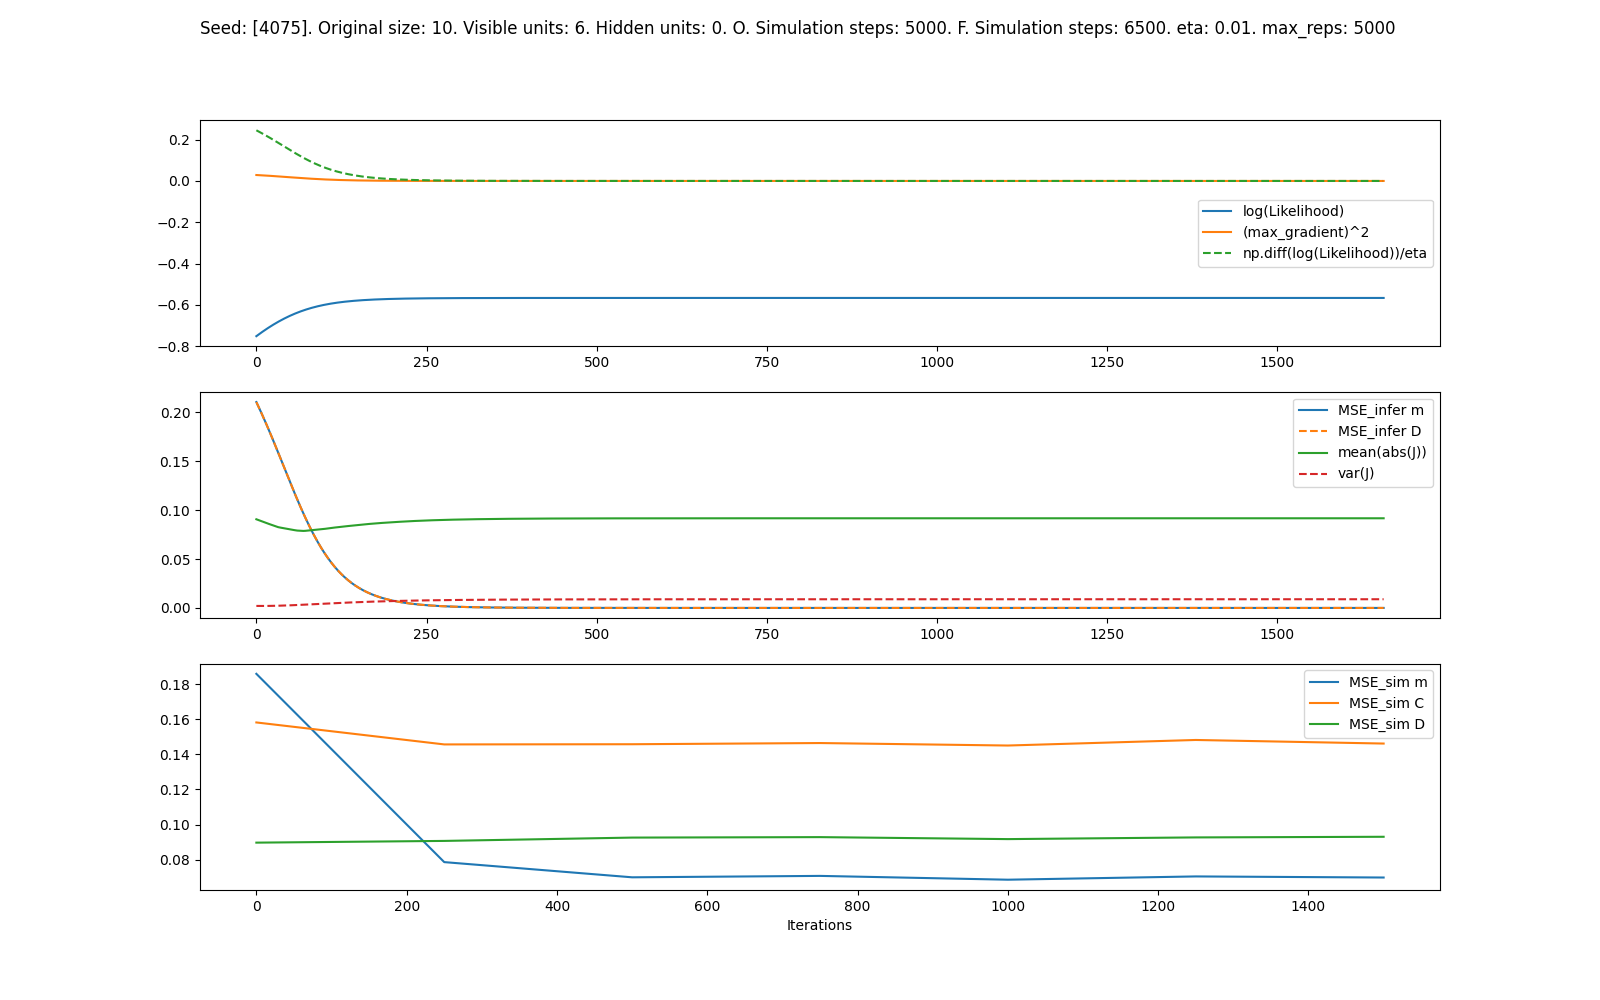
\includegraphics[width=0.7\linewidth]{images/sqrt_size/[4075]_10_6_0_5000_6500_eta001_5000_100.png}
\caption{Seed: 4075. Standard Ising model. Top: logarithm of the likelihood, square of the maximum gradient and difference of the likelihood between consecutive time-steps. Middle: MSE of m and D during inference and evolution of the behavior of $\*J$. Bottom: MSE of m, D and D after the simulations.}
\end{figure}


\begin{figure}[!htb]
    \centering
    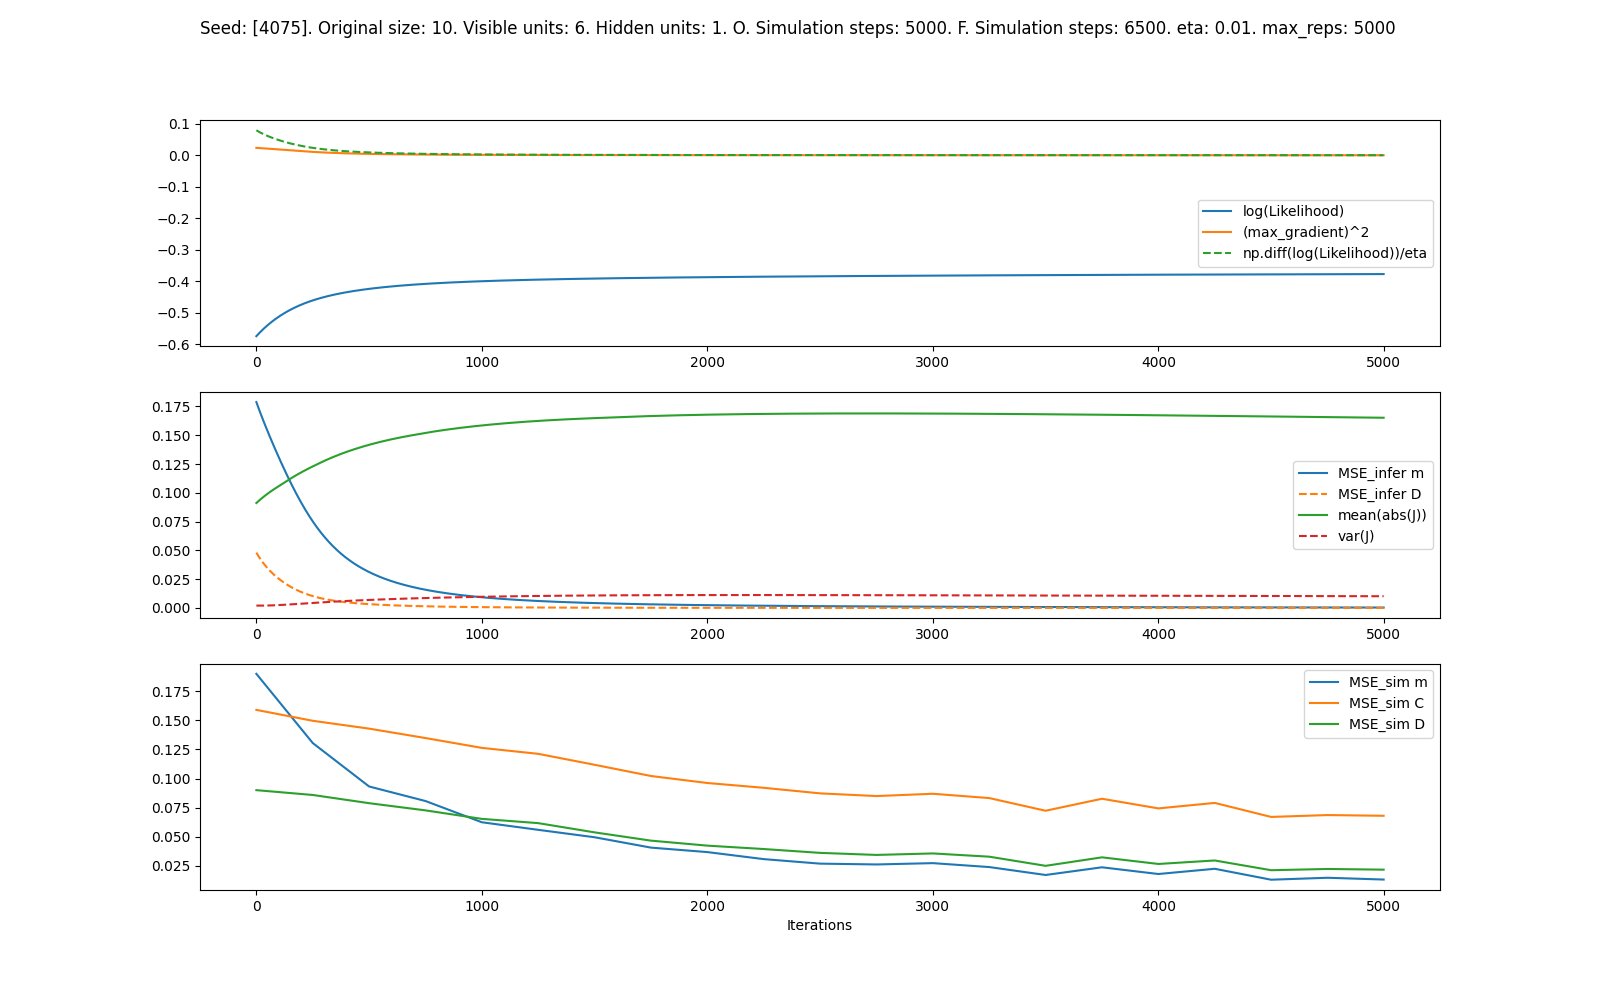
\includegraphics[width=0.7\linewidth]{images/sqrt_size/[4075]_10_6_1_5000_6500_eta001_5000_100.png}
\caption{Seed: 4075. Kinetic Ising model with 1 hidden unit. Top: logarithm of the likelihood, square of the maximum gradient and difference of the likelihood between consecutive time-steps. Middle: MSE of m and D during inference and evolution of the behavior of $\*J$. Bottom: MSE of m, D and D after the simulations.}
\end{figure}





\end{document}

        